\cleardoublepage\documentclass[../main.tex]{subfiles}
\begin{document}
\chapter{TIKZ}
\section{Comandos}Dentro do ambiente, podem ser usados, dentre outros, os comandos:
\begin{compactenum}[a)]
\item \verb|\draw| – para desenhar linhas
\item \verb|\fill| – para preencher ´areas com cores s´olidas
\item \verb|\verb|\shade| – para preencher ´areas com cores gradientes
\item \clip – para preencher ´areas com cores s´olidas
\end{compactenum}
\section{Desenhos básicos}
\subsection{Linhas}
\tikz \draw (0, 0) -- (1, 1);
\tikz \draw[blue, dotted,  ultra thick] (0, 0) -- (1, 1);
\verb|ultra tick| define a largura da linha
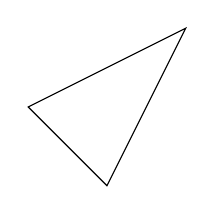
\begin{tikzpicture}
\draw (0,1)--(1,0)--(2,2)--cycle;
\end{tikzpicture}

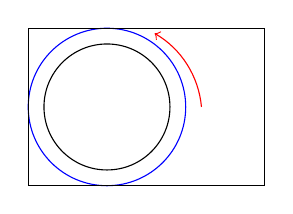
\begin{tikzpicture}
%círculo com centro na origem e raio unitário
 \draw[blue] (0,0) circle (1);
%também podemos usar unidades de medida
 \draw (0,0) circle (8mm);
%retângulo
 \draw (-1,-1) rectangle (2,1);%retângulo de largura dois e altura um
%arco
 \draw[->,red] (1.2,0) arc (5:60:1.2); %(x,y) são coordenadas
\end{tikzpicture}
%curvas
\section{Funções}
%gráfico de função
\begin{tikzpicture}
  \draw[->] (-3,0) -- (3,0);
  \draw[->] (0,-1) -- (0,4);
  \draw[blue,smooth,samples=100,domain=-2.0:2.0] plot(\x,{(\x)^2});
\end{tikzpicture}

%função seno
\begin{tikzpicture}
\draw[->] (-2*pi-0.5,0) -- (2*pi+0.5,0) node[right] {$x$};
\draw[->] (0,-1.5) -- (0, 1.5) node[above] {$y$};
\draw[blue, domain=-2*pi:2*pi, smooth] plot (\x,{sin(\x r)});
\end{tikzpicture}

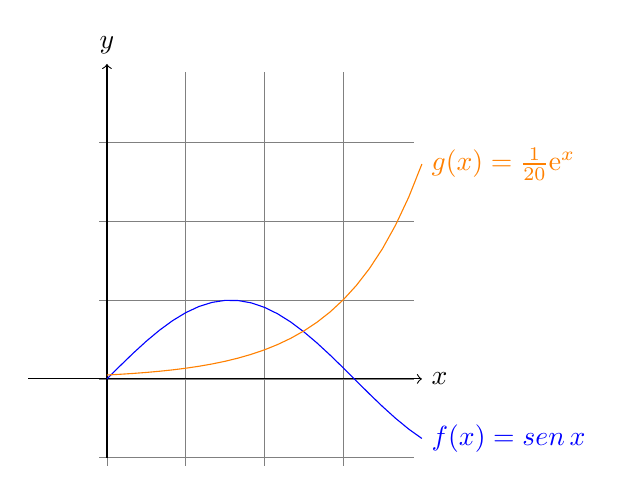
\begin{tikzpicture}[domain=0:4]
\draw[help lines] (-0.1,-1.1) grid (3.9,3.9);
\draw[->] (-1,0) -- (4,0) node[right] {$x$};
\draw[->] (0,-1) -- (0, 4) node[above] {$y$};
\draw[blue] plot (\x,{sin(\x r)}) node[right] {$f(x) = \text{sen\,}x$};
\draw[orange] plot (\x,{0.05*exp(\x)}) node[right]
{$g(x) = \frac{1}{20} \mathrm e^x$};
\end{tikzpicture}

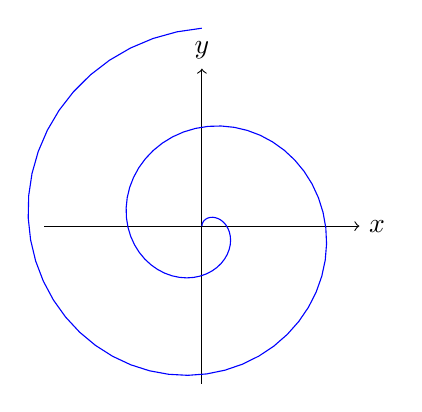
\begin{tikzpicture}[scale=0.4]
\draw[->] (-5,0) -- (5,0) node[right] {$x$};
\draw[->] (0,-5) -- (0,5) node[above] {$y$};
\draw[scale=0.5,blue, samples=100, domain=0:4*pi]
plot ({\x*sin(\x r)},{\x*cos(\x r)});
\end{tikzpicture}



\section{Desenhos mais elaborados}
\begin{center}
\begin{tikzpicture}[domain=-3.2:3.2]
%\draw[dotted] (-3.2,-1.2) grid (3.2,1.2);
\draw[->] (-3.5,0) -- (6.5,0) node[right] {$x$};
\draw[->] (0,-5.2) -- (0,2.2) node[above] {$y$};
% O angulo padrão será em graus. Para usar em radianos, acrescente ” r” no parametro da
funcao trigonometrica
\draw[smooth,color=blue,domain=-pi-0.1:pi+0.1] plot (\x,{sin(\x r)}) node[above] {$f(x)
=\mathrm{sen}(x)$};
% Curvas em coordenada polar. O angulo padrao sera em graus. A funcao deg() converte
radiano para grau (é mesmo que colocar sufixo r)
\draw[smooth,color=red,domain=0:2*pi] plot ({deg(\x)}:\x) node[above] {$\rho(\theta) =\
theta$};
% curvas parametricas.
% podera especificar o nome da variavel em vez de usar o padrao \x
\draw[smooth,color=green,domain=-1.8:1.8,variable=\t] plot ({cosh(\t)},{sinh(\t)}) node[
above]{$\text{ramo de }x^2-y^2=1$};
\end{tikzpicture}
\end{center}
\section{Matriz}
\begin{center} %MATRIZ
\begin{tikzpicture}
\matrix (A) [matrix of math nodes,left delimiter=[,right delimiter={]} ]
{ 1 & 2 & -1 & 5 \\
0 & |[draw=red,circle]|3 & 2 & 1 \\
0 & -2 & \phantom{-}2 & -4 \\
};
% separando a matriz da parte aumentada
\draw[thick,dashed,blue] (A-1-3.north east) -- (A-3-3.south east);
% limitando a parte escalonada
\draw[thick,dotted,blue] (A-2-1.north west) -- (A-2-1.north east) -- (A-3-1.south
east);
% onde vai colocar a seta para piv\^o
\coordinate (P) at ($(A-2-1)!-2!(A-2-2)$);
\coordinate (Q) at ($(A-2-1)!-1.3!(A-2-2)$);
% colocando a seta na linha de piv\^o
\draw[->] (P) -- (Q);
\node at ($(P)!-1.2!(Q)$) {piv\^o};
\end{tikzpicture}
\end{center}

%==================================================

\chapter{Caixas Personalizadas}
%++++++ cAIXAS DE TEXTO+++++++++
%CAIXA SIMPLES PADRÃO
\begin{tcolorbox} %
This is a \textbf{tcolorbox}.
\end{tcolorbox}\vspace{1CM}


\section{CAIXA DIVIDIDA COM UMA LINHA}
%CAIXA DIVIDIDA COM UMA LINHA
\begin{tcolorbox}
This is another \textbf{tcolorbox}.
\tcblower
Here, you see the lower part of the box.
\end{tcolorbox}\vspace{1cm}


CAIXA COM TÍTULO DE COR DIFERENTE\\
%CAIXA COM TÍTULO DE COR DIFERENTE
\begin{tcolorbox}[colback=red!5!white,colframe=red!95!black,fonttitle=\bfseries,title=TITULO]
This is another \textbf{tcolorbox}.
\tcblower
Here, you see the lower part of the box.
\end{tcolorbox}\vspace{1CM}

DEFININDO COR DE TEXTO DE ACORDO COM A PARTE DA CAIXA
\begin{tcolorbox}[colupper=red!75!black] %PARA CAIXA DE BAIXO=COLLOWER, PARA TODOS: COLTEXT
This is a \textbf{tcolorbox}.
\tcblower
This is the lower part.
\end{tcolorbox}

CAIXA COM TÍTULO INVISÍVEL OU VISÍVEL
%CAIXA COM TÍTULO INVISÍVEL OU VISÍVEL
\begin{tcolorbox}[title=TITULO VISÍVEL OU INVISISIVEL,
titlebox=invisible,colback=red!5!white,coltitle=white]
This is a \textbf{tcolorbox}.
\end{tcolorbox}

%OUTRO ESTILO COM 
\begin{tcolorbox}[upperbox=invisible,colback=white,lowerbox=visible]%OPÇÕES=visible, invisibel, ignored (separa a caixa uma da outra)
This is a \textbf{tcolorbox} (but invisible).
\tcblower
This is the lower part.
\end{tcolorbox}\vspace{1CM}

CONTEÚDO SALVO PARA SER USADO DEPOIS
%CONTEÚDO SALVO PARA SER USADO DEPOIS
%============================================
\begin{tcolorbox}[saveto=\jobname_mysave2.tex]%define o conteúdo salvo
This is a \textbf{tcolorbox}.
\tcblower
This is the lower part.
\end{tcolorbox}
Now, we load the saved text:
\begin{tcolorbox}[colframe=red,colback=red!10,
coltitle=black,colbacktitle=red!20,sidebyside,title=Here we see the saved content including the lower part]
\input{\jobname_mysave2.tex}%CARREGA O CONTEÚDO SALVO
\end{tcolorbox}
\section{SALVANDO SÓ A PARTE DE BAIXO}
%SALVA O CONTEÚDO SÓ DA PARTE INFERIOR PARA USAR DEPOIS
\begin{tcolorbox}[lowerbox=invisible,savelowerto=\jobname_bspsave.tex,colback=white]
This is a \textbf{tcolorbox}.
\tcblower
This is the lower part which may be quite complex:
$\displaystyle f(x)=\frac{1+x^2}{1-x^2}$.
\end{tcolorbox}
Now, we load the saved text:\\
\input{\jobname_bspsave.tex}\\
\section{ALVA E IGNORA A PARTE DE BAIXO PARA USAR DEPOIS COM O PRÓPRIO AMBIENTE}
%SALVA E IGNORA A PARTE DE BAIXO PARA USAR DEPOIS COM O PRÓPRIO AMBIENTE
\newtcolorbox{mybox}[1]{%
savelowerto=\jobname_bspsave2.tex,lowerbox=ignored,
colback=red!5!white,colframe=red!75!black,fonttitle=\bfseries,
title=#1}%
\begin{mybox}{My Example}
Upper part.
\tcblower
Saved lower part!
\end{mybox}
Now, the saved part is used:
\begin{tcolorbox}[colback=green!5]
\input{\jobname_bspsave2.tex}
\end{tcolorbox}
%==============================================

\section{VÁRIAS CAIXAS acopladas}
%VÁRIAS CAIXAS acopladas
\tcbset{colback=green!10!white,fonttitle=\bfseries}%COR DO FUNDO DA PRIMEIRA CAIXA (PRINCIPAL
\tcbsetforeverylayer{colframe=red!5!black}%DEFINE A COR DO TÍTULO PARA TODAS AS SUBCAIXAS
\begin{tcolorbox}[title=All options for this box]
This is a tcolorbox.\par\medskip
\begin{tcolorbox}[title=Nested box]
Note that this nested box has a red frame but no green background.
\end{tcolorbox}
\end{tcolorbox}


DEFININDO AS PRÓPRIAS CAIXAS PERSONALIZÁVEIS
%CRIANDO O PRÓPRIO AMBIENTE BASEADO NO TCOLORBOX
\newtcolorbox{mybox2}[1]{colback=red!5!white,
colframe=red!75!black,fonttitle=\bfseries,title=#1}
\begin{mybox2}{TITULO}
ESTA É MINHA CAIXA COM TÍTULO\\
\end{mybox2}\vspace{1cm}

\section{DEFININDO UM AMBIENTE BASEADO NO TCOLOR BOX PARA EXEMPLOS NUMERADO PELA SEÇÃO e com quebra}
\subsection{Um primeiro exemplo}
%DEFININDO UM AMBIENTE BASEADO NO TCOLOR BOX PARA EXEMPLOS NUMERADO PELA SEÇÃO
\newtcolorbox[auto counter,number within=section]{pabox}[2][]{%
before=\par\medskip,parbox=false,boxsep=3pt,left=3pt,right=3mm,top=4pt,pad at break*=0mm,vfill before first,
breakable,colback=red!1!white,colframe=red!75!black,fonttitle=\Large\bfseries,
title=Examplo.~\thetcbcounter: #2,#1} %colocar no preâmbulo

\begin{pabox}[fonttitle=\sffamily\bfseries\large,colbacktitle=black!20!white,coltitle=red]{Hello there} %SE TIRAR AS OPÇÕES FICA O PADRÃO DEFINIDO ACIMA
This is my own box with a mandatory
numbered title and options. This isdddada my own box with a mandatory
numbered title and options.This is my own box with a mandatory
numbered title and options.
\lipsum[2-5]
\end{pabox}
\subsection{Outro exemplo com overlay}
%\newcounter{example} %COLOCAR NO PREAMBULO
\colorlet{colexam}{red!75!black}
\newtcolorbox[auto counter,number within=section]{myexample}{%
empty,title={Examplo \thetcbcounter},attach boxed title to top left,
boxed title style={empty,size=minimal,toprule=2pt,top=4pt,
overlay={\draw[colexam,line width=2pt]
([yshift=-1pt]frame.north west)--([yshift=-1pt]frame.north east);}},
coltitle=colexam,fonttitle=\Large\bfseries,
before=\par\medskip\noindent,parbox=false,boxsep=0pt,left=0pt,right=3mm,top=4pt,
breakable,pad at break*=0mm,vfill before first,
overlay unbroken={\draw[colexam,line width=1pt]
([yshift=-1pt]title.north east)--([xshift=-0.5pt,yshift=-1pt]title.north-|frame.east)
--([xshift=-0.5pt]frame.south east)--(frame.south west); },
overlay first={\draw[colexam,line width=1pt]
([yshift=-1pt]title.north east)--([xshift=-0.5pt,yshift=-1pt]title.north-|frame.east)
--([xshift=-0.5pt]frame.south east); },
overlay middle={\draw[colexam,line width=1pt] ([xshift=-0.5pt]frame.north east)
--([xshift=-0.5pt]frame.south east); },
overlay last={\draw[colexam,line width=1pt] ([xshift=-0.5pt]frame.north east)
--([xshift=-0.5pt]frame.south east)--(frame.south west);},%
}
\begin{myexample}
\lipsum[1]\par
\begin{myexample}
Testando 
\end{myexample}
\end{myexample}
\begin{myexample}
\lipsum[2-5]
\end{myexample}
\lipsum[12]% following text




\section{Caixas definidas próprias de exemplos e exercícios com respostas gravadas}
\subsection{código postado abaixo-oculto}
%DEFININDO O AMBIENTE EXERCICIO
\NewTColorBox[auto counter,number within=section]{exercise}{+!O{}}{%
enhanced,colframe=green!20!black,colback=yellow!10!white,coltitle=green!40!black,
fonttitle=\bfseries,
underlay={\begin{tcbclipinterior}
\shade[inner color=green!80!yellow,outer color=yellow!10!white]
(interior.north west) circle (2cm);
\draw[help lines,step=5mm,yellow!80!black,shift={(interior.north west)}]
(interior.south west) grid (interior.north east);
\end{tcbclipinterior}},
title={Exercício~\thetcbcounter:},
label={exercise@\thetcbcounter},
attach title to upper=\quad,
after upper={\par\hfill\textcolor{green!40!black}%
{\itshape Solução na página~\pageref{solution@\thetcbcounter}}},
lowerbox=ignored,
savelowerto=exercise-\thetcbcounter.tex,
record={\string\solution{\thetcbcounter}{exercise-\thetcbcounter.tex}},
#1
}   

%DEFININDO O AMBIENTE SOLUÇÃO 
\NewTotalTColorBox{\solution}{mm}{%
enhanced,colframe=red!20!black,colback=yellow!10!white,coltitle=red!40!black,
fonttitle=\bfseries,
underlay={\begin{tcbclipinterior}
\shade[inner color=red!50!yellow,outer color=yellow!10!white]
(interior.north west) circle (2cm);
\draw[help lines,step=5mm,yellow!80!black,shift={(interior.north west)}]
(interior.south west) grid (interior.north east);
\end{tcbclipinterior}},
title={SSolução do Exercício~\ref{exercise@#1} na página~\pageref{exercise@#1}:},
phantomlabel={solution@#1},
attach title to upper=\par,
}{\input{#2}}

\tcbset{no solution/.style={no recording,after upper=}}
\tcbstartrecording\relax

\subsection{Aplicando...}
\begin{exercise}
Compute the derivative of the following function:
\begin{equation*}
f(x)=\sin((\sin x)^2)
\end{equation*}

\tcblower
The derivative is:
\begin{align*}
f'(x) &= \left( \sin((\sin x)^2) \right)'
=\cos((\sin x)^2) 2\sin x \cos x.
\end{align*}
\end{exercise}

\begin{exercise}[no solution]
It holds:
\begin{equation*}
\frac{d}{dx}\left(\ln|x|\right) = \frac{1}{x}.
\end{equation*}
\end{exercise}

\begin{exercise}
Compute the derivative of the following function:
\begin{equation*}
f(x)=(\sin(\sin x))^2
\end{equation*}
\tcblower
The derivative is:
\begin{align*}
f'(x) &= \left( (\sin(\sin x))^2 \right)'
=2\sin(\sin x)\cos(\sin x)\cos x.
\end{align*}
\end{exercise}
\begin{exercise}
Compute the derivative of the following function:
\begin{equation*}
f(x)=\sqrt{x^3-6x^2+2x}
\end{equation*}
\tcblower
The derivative is:
\begin{align*}
f'(x) &= \left( \sqrt{x^3-6x^2+2x} \right)'
= \frac{3x^2-12x+2}{2\sqrt{x^3-6x^2+2x}}.
\end{align*}
\end{exercise}
\begin{exercise}
Compute the derivative of the following function:
\begin{equation*}
f(x)=\left(\frac{2+3x}{1-2x}\right)^3
\end{equation*}
\tcblower
The derivative is:
\begin{align*}
f'(x) &= \left( \left(\frac{2+3x}{1-2x}\right)^3 \right)'
= 3 \left(\frac{2+3x}{1-2x}\right)^2 \frac{(1-2x)3-(2+3x)(-2)}{(1-2x)^2}
= \frac{21(2+3x)^2}{(1-2x)^4}.
\end{align*}
\end{exercise}

\begin{exercise}
Compute the derivative of the following function:
\begin{equation*}
f(x)=\frac{\cos x}{(\tan 2x)^2}
\end{equation*}
\tcblower
The derivative is:
\begin{align*}
f'(x) &= \left( \frac{\cos x}{(\tan 2x)^2} \right)'
= \left( \frac{\cos x (\cos 2x)^2}{(\sin 2x)^2} \right)'\\
&= \frac{(\sin 2x)^2 [(-\sin x)(\cos 2x)^2+(\cos x)4\cos 2x (-\sin 2x)]
- \cos x (\cos 2x)^2 4\sin 2x \cos 2x}{(\sin 2x)^4}\\
&= -\frac{\cos(2x) [\sin x \sin 2x \cos 2x+ 4\cos x(\sin 2x)^2
+ 4 \cos x (\cos 2x)^2]}{(\sin 2x)^3}\\
&= -\frac{\cos(2x) [\sin x \sin 2x \cos 2x+ 4\cos x]}{(\sin 2x)^3}.
\end{align*}
\end{exercise}
\begin{exercise}
Compute the derivative of the following function:
\begin{equation*}
f(x)=\cos((2x^2+3)^3)
\end{equation*}
\tcblower
The derivative is:
\begin{align*}
f'(x) &= \left( \cos((2x^2+3)^3) \right)'
=-\sin((2x^2+3)^3) 3(2x^2+3)^2 2\cdot 2x\\
&=-12x(2x^2+3)^2\sin((2x^2+3)^3).
\end{align*}
\end{exercise}
\begin{exercise}
Compute the derivative of the following function:
\begin{equation*}
f(x)=(x^2+1)\sqrt{x^4+1}
\end{equation*}
\tcblower
The derivative is:
\begin{align*}
f'(x) &= \left( (x^2+1)\sqrt{x^4+1} \right)'
= 2x\sqrt{x^4+1} + \frac{2x^3(x^2+1)}{\sqrt{x^4+1}}.
\end{align*}
\end{exercise}
\tcbstoprecording %FECHANDO A GRAVAÇÃO

\subsubsection{apresentando as soluções}
\tcbinputrecords





\section{caixas e subcaixas}
CAIXAS E SUBCAIXAS
%caixas e subcaixas
\begin{tcolorbox}[title=My title,
colback=red!5!white,
colframe=red!75!black,
colbacktitle=yellow!50!red,
coltitle=red!25!black,
fonttitle=\bfseries]
This is a \textbf{tcolorbox}.
\tcbsubtitle[before skip=\baselineskip]%
{My subtitle}
Further text.
\end{tcolorbox}

%OUTRO EXEMPLO ALTERANDO O ESTILO DAS SUBCAIXAS
\begin{tcolorbox}[title=My title,
colback=red!5!white,
colframe=red!75!black,
colbacktitle=yellow!50!red,
coltitle=red!25!black,
fonttitle=\bfseries,
subtitle style={boxrule=0.4pt,
colback=yellow!50!red!25!white} ]
This is a \textbf{tcolorbox}.
\tcbsubtitle{My subtitle}
Further text.
\tcbsubtitle{Second subtitle}
Further text.
\end{tcolorbox}\vspace{1cm}

 DEFININDO O TAMANHO DAS CAIXAS\\
%DEFININDO O TAMANHO DAS CAIXAS
\begin{tcolorbox}[width=\linewidth/2,opacityframe=0.5,opacityback=0.5]
This is a \textbf{tcolorbox}.
\end{tcolorbox}
\vspace{1CM}

DEFININDO TAMANHO NAS LATERAIS, EM CIMA ETC
%TAMANHO DAS LATERAIS, EM CIMA ETC
\tcbset{colback=red!5!white,colframe=red!75!black} 
\begin{tcolorbox}[leftrule=3mm] %OUTHER:TOPRULE, RIGHTRULE, BOTTOMRULE
This is a \textbf{tcolorbox}.
\end{tcolorbox}

\tcbset{colback=red!5!white,colframe=red!75!black,colbacktitle=red!90!black}
\begin{tcolorbox}[titlerule=2.5mm,title=This is the title]
This is a \textbf{tcolorbox}.
\end{tcolorbox}
\begin{tcolorbox}[boxrule=3mm]
This is a \textbf{tcolorbox}.
\end{tcolorbox}
\vspace{1CM}

%DEFININDO O QUANTO ARRENDDADA FICA
\begin{tcolorbox}[arc=0mm]
This is a \textbf{tcolorbox}.
\end{tcolorbox}
\begin{tcolorbox}[arc=3mm]
This is a \textbf{tcolorbox}.
\end{tcolorbox}

\vspace{1CM}
DEFININDO DE FORMA CIRCULAR E OUTRAS
\begin{tcolorbox}[width=3cm,
colback=red!5!white,
colframe=red!75!black,
halign=center,valign=center,
square,circular arc]
This is a \textbf{tcolorbox}.
\end{tcolorbox}



\begin{tcolorbox}[auto outer arc,
width=2.2cm,octogon arc,
colback=white,colframe=red,
halign=center,valign=center,
square,arc is angular
    ]
\begin{tcolorbox}[size=minimal,auto outer arc,
width=2.1cm,octogon arc,
colback=red,colframe=white,colupper=white,
fontupper=\fontsize{7mm}{7mm}\selectfont\bfseries\sffamily,
halign=center,valign=center,square,arc is angular]
STOP
\end{tcolorbox}
\end{tcolorbox}

\vspace{2CM}
\begin{tcolorbox}[size=minimal,auto outer arc,
width=2.1cm,octogon arc,
colback=red,colframe=white,colupper=white,
fontupper=\fontsize{7mm}{7mm}\selectfont\bfseries\sffamily,
halign=center,valign=center,
square,arc is angular,
borderline={1.2mm}{5mm}{red}]
STOP
\end{tcolorbox}
ESTILO CONTINUAÇÃO 
{\tcbset{after upper={\par\hfill\textit{Read more next week}},
colback=red!5!white,colframe=red!75!black,fonttitle=\bfseries}
\begin{tcolorbox}[title=My title]
This is a \textbf{tcolorbox}.
\end{tcolorbox}\vspace{1CM}}



\section{ESTILO CAPA-TALVEZ}
\begin{tcolorbox}[colback=red!5!white,colframe=red!75!black,fonttitle=\bfseries,
height=8cm,text fill,
title=My filled box]
This is a \textbf{tcolorbox}.
\par\vfill
\begin{center}
My middle text.
\end{center}
\par\vfill
This is the end of my box.
\end{tcolorbox}
\vspace{1CM}



\section{TABELAS}
\tcbset{enhanced,fonttitle=\bfseries\large,fontupper=\normalsize\sffamily,
colback=yellow!10!white,colframe=red!50!black,colbacktitle=Salmon!30!white,
coltitle=black,center title}
\begin{tcolorbox}[tabulars={@{\extracolsep{\fill}\hspace{5mm}}lrrrrr@{\hspace{5mm}}},
boxrule=0.5pt,title=My table]
Group & One & Two & Three & Four & Sum\\\hline\hline
Red & 1000.00 & 2000.00 & 3000.00 & 4000.00 & 10000.00\\\hline
Green & 2000.00 & 3000.00 & 4000.00 & 5000.00 & 14000.00\\\hline
Blue & 3000.00 & 4000.00 & 5000.00 & 6000.00 & 18000.00\\\hline\hline
Sum & 6000.00 & 9000.00 & 12000.00 & 15000.00 & 42000.00
\end{tcolorbox}
COM ESPAÇAMENTO EXTRA ENTRE LINHAS
\tcbset{enhanced,fonttitle=\bfseries\large,fontupper=\normalsize\sffamily,
colback=yellow!10!white,colframe=red!50!black,colbacktitle=Salmon!30!white,
coltitle=black,center title}
\begin{tcolorbox}[tabulars*={\arrayrulewidth0.5mm\renewcommand\arraystretch{1.4}}%
{@{\extracolsep{\fill}\hspace{20mm}}lll@{\hspace{20mm}}},
title=My table]
One & Two & Three \\\hline\hline
1000.00 & 2000.00 & 3000.00\\\hline
2000.00 & 3000.00 & 4000.00
\end{tcolorbox}
\vspace{1CM}
\section{UTILIZANDO O TICKZ}
{
\begin{tcolorbox}[tikz upper,fonttitle=\bfseries,colback=white,colframe=black,
title=\ tikzname\ drawing]
texto exemplo
\path[fill=yellow,draw=yellow!75!red] (0,0) circle (1cm);
\fill[red] (45:5mm) circle (1mm);
\fill[red] (135:5mm) circle (1mm);
\draw[line width=1mm,red] (215:5mm) arc (215:325:5mm);
\end{tcolorbox}
}
{
\begin{tcblisting}{tikz lower,listing side text,fonttitle=\bfseries,
bicolor,colback=Blue!10!white,colbacklower=white,colframe=black,
righthand width=3cm,title=tikzname drawing}
\path[fill=yellow,draw=yellow!75!red]
(0,0) circle (1cm);
\fill[red] (45:5mm) circle (1mm);
\fill[red] (135:5mm) circle (1mm);
\draw[line width=1mm,red]
(215:5mm) arc (215:325:5mm);
\end{tcblisting}
}
{
\tcbset{frogbox/.style={enhanced,colback=green!10,colframe=green!65!black,
enlarge top by=5.5mm,
overlay={\foreach \x in {2cm,3.5cm} {
\begin{scope}[shift={([xshift=\x]frame.north west)}]
\path[draw=green!65!black,fill=green!10,line width=1mm] (0,0) arc (0:180:5mm);
\path[fill=black] (-0.2,0) arc (0:180:1mm);
\end{scope}}}}}
\begin{tcolorbox}[frogbox,title=My title]
This is a \textbf{tcolorbox}.
\end{tcolorbox}}



\section{Estilos numeração ou itemize}
\begin{tcbitemize}[size=small,colframe=red!50!black,colback=red!10!white,
raster odd column/.style={colframe=blue!50!black,colback=blue!10!white}]
\tcbitem One
\tcbitem Two
\tcbitem Three
\tcbitem Four
\end{tcbitemize}
\section{outros estilos}
\newtcolorbox{caixadex}[2][]{enhanced,skin=enhancedlast jigsaw,
attach boxed title to top left={xshift=-4mm,yshift=-0.5mm},
fonttitle=\bfseries\sffamily,varwidth boxed title=0.7\linewidth,
colbacktitle=blue!45!white,colframe=red!50!black,
interior style={top color=blue!10!white,bottom color=red!10!white},
boxed title style={empty,arc=0pt,outer arc=0pt,boxrule=0pt},
underlay boxed title={
\fill[blue!45!white] (title.north west) -- (title.north east)
-- +(\tcboxedtitleheight-1mm,-\tcboxedtitleheight+1mm)
-- ([xshift=4mm,yshift=0.5mm]frame.north east) -- +(0mm,-1mm)
-- (title.south west) -- cycle;
\fill[blue!45!white!50!black] ([yshift=-0.5mm]frame.north west)
-- +(-0.4,0) -- +(0,-0.3) -- cycle;
\fill[blue!45!white!50!black] ([yshift=-0.5mm]frame.north east)
-- +(0,-0.3) -- +(0.4,0) -- cycle; },
title={#2},#1}
\begin{caixadex}{My title}
\lipsum[2]
\end{caixadex}
\newtcolorbox{caixadex2}[2][]{enhanced,
before skip=2mm,after skip=2mm,
colback=black!5,colframe=black!50,boxrule=0.2mm,
attach boxed title to top left={xshift=1cm,yshift*=1mm-\tcboxedtitleheight},
varwidth boxed title*=-3cm,
boxed title style={frame code={
\path[fill=tcbcolback!30!black]
([yshift=-1mm,xshift=-1mm]frame.north west)
arc[start angle=0,end angle=180,radius=1mm]
([yshift=-1mm,xshift=1mm]frame.north east)
arc[start angle=180,end angle=0,radius=1mm];
\path[left color=tcbcolback!60!black,right color=tcbcolback!60!black,
middle color=tcbcolback!80!black]
([xshift=-2mm]frame.north west) -- ([xshift=2mm]frame.north east)
[rounded corners=1mm]-- ([xshift=1mm,yshift=-1mm]frame.north east)
-- (frame.south east) -- (frame.south west)
-- ([xshift=-1mm,yshift=-1mm]frame.north west)
[sharp corners]-- cycle;
},interior engine=empty,
},
fonttitle=\bfseries,
title={#2},#1}
\begin{caixadex2}[colbacktitle=green]{My title}
\lipsum[2]
\end{caixadex2}
\begin{caixadex2}[colbacktitle=red]{My title}
\lipsum[3]
\end{caixadex2}

\tcbset{colback=red!5!white,colframe=red!75!black,fonttitle=\bfseries}
\begin{tcolorbox}[enhanced,title=MARCA D'AGUA,watermark text=My Watermark]
\lipsum[1]
\tcblower
\lipsum[2]
\end{tcolorbox}

\begin{tcolorbox}[enhanced,title=My title,
watermark tikz={\draw[line width=2mm] circle (1cm)
node{\fontfamily{ptm}\fontseries{b}\fontsize{20mm}{20mm}\selectfont ?};},watermark color=yellow!80!red]
\lipsum[1]
\tcblower
\lipsum[2]
\end{tcolorbox}

\section{ajustes extras-Skins and Drawing}
\tcbset{colback=red!5!white,colframe=red!75!black,fonttitle=\bfseries}
\begin{tcolorbox}[enhanced,title=My title,segmentation code={
\path[top color=red!5!white,bottom color=red!5!white,middle color=blue]
(segmentation.south west) rectangle (segmentation.north east);}]
This is a \textbf{tcolorbox}.
\tcblower
This is the lower part.
\end{tcolorbox}



\tcbset{colback=red!5!white,colframe=yellow!75!black,
width=(\linewidth-8mm)/2,before=,after=\hfill,equal height group=ske}
\begin{tcolorbox}[adjusted title=My title]
This is my content.
\end{tcolorbox}
\begin{tcolorbox}[skin=beamer,beamer,adjusted title=OLHA A DIFERENÇA]
This is my content.
\end{tcolorbox}


\section{VÁRIAS CAIXAS EM LINHA}
%VÁRIAS CAIXAS EM LINHA
\tcbset{colback=White,arc=0mm,width=(\linewidth-4pt)/4, %O ÚLTIMO N. É QUANTAS CAIXAS POR LINHA
equal height group=AT,before=,after=\hfill,fonttitle=\bfseries}
The following titles are not adjusted:\\
\foreach \n in {xxx,ggg,AAAAAAAAAAAAAAAAAAADDDDDDDDDDA,\"Agypten}
{\begin{tcolorbox}[title=\n,colframe=red!75!black]
Some contentSome contentSome\end{tcolorbox}}

Now, we try again with adjusted titles:\\
\foreach \n in {xxx,ggg,AAA} %O TÍTULO DAS CIAXAS DEFINE A QUANTIDADE DELAS
{\begin{tcolorbox}[adjusted title=\n,colframe=blue!75!black]
Some content.\end{tcolorbox}}\\
\vspace{1cm}

VÁRIAS CAIXAS DISTRIBUIDAS\\
Every line is inside an equal height group:
\begin{tcbraster}[raster equal height=rows,
title=Box \thetcbrasternum,
enhanced,size=small,colframe=red!50!black,colback=red!10!white]
\begin{tcolorbox}First line\\second line\\
The height of this box rules.\end{tcolorbox}
\begin{tcolorbox}[use height from group]Test\end{tcolorbox}
\begin{tcolorbox}[use height from group]
First line\\second line\end{tcolorbox}
\begin{tcolorbox}The height of this box rules.\end{tcolorbox}
\end{tcbraster}
\end{document}

